\documentclass[8pt,aspectratio=169]{beamer}
\usetheme{Madrid}
\usepackage{graphicx}
\usepackage{booktabs}
\usepackage{adjustbox}
\usepackage{multicol}
\usepackage{amsmath}
\usepackage{amssymb}
\usepackage{tikz}
\usepackage{hyperref}
\usepackage{algorithm}
\usepackage{algorithmic}
\usepackage{colortbl}
\usepackage{pgfplots}
\pgfplotsset{compat=1.18}

% TikZ libraries for comics, diagrams, stakeholder maps
\usetikzlibrary{arrows.meta,positioning,shapes.callouts,shapes.geometric,decorations.pathreplacing}

% Color definitions
\definecolor{mlblue}{RGB}{0,102,204}
\definecolor{mlpurple}{RGB}{51,51,178}
\definecolor{mllavender}{RGB}{173,173,224}
\definecolor{mllavender2}{RGB}{193,193,232}
\definecolor{mllavender3}{RGB}{204,204,235}
\definecolor{mllavender4}{RGB}{214,214,239}
\definecolor{mlorange}{RGB}{255, 127, 14}
\definecolor{mlgreen}{RGB}{44, 160, 44}
\definecolor{mlred}{RGB}{214, 39, 40}
\definecolor{mlgray}{RGB}{127, 127, 127}
\definecolor{lightgray}{RGB}{240, 240, 240}
\definecolor{midgray}{RGB}{180, 180, 180}

% NEW COLORS for mini-lecture
\definecolor{dfteal}{RGB}{0,128,128}
\definecolor{dfred}{RGB}{180,30,30}

% Backward compatibility
\colorlet{MLPurple}{mlpurple}
\colorlet{MLBlue}{mlblue}
\colorlet{MLOrange}{mlorange}
\colorlet{MLGreen}{mlgreen}
\colorlet{MLRed}{mlred}
\colorlet{MLLavender}{mllavender}
\colorlet{MLGray}{mlgray}

% Theme colors (exact Madrid settings)
\setbeamercolor{palette primary}{bg=mllavender3,fg=mlpurple}
\setbeamercolor{palette secondary}{bg=mllavender2,fg=mlpurple}
\setbeamercolor{palette tertiary}{bg=mllavender,fg=white}
\setbeamercolor{palette quaternary}{bg=mlpurple,fg=white}
\setbeamercolor{structure}{fg=mlpurple}
\setbeamercolor{section in toc}{fg=mlpurple}
\setbeamercolor{subsection in toc}{fg=mlblue}
\setbeamercolor{title}{fg=mlpurple}
\setbeamercolor{frametitle}{fg=mlpurple,bg=mllavender3}
\setbeamercolor{block title}{bg=mllavender2,fg=mlpurple}
\setbeamercolor{block body}{bg=mllavender4,fg=black}
\setbeamertemplate{navigation symbols}{}
\setbeamertemplate{itemize items}[circle]
\setbeamertemplate{enumerate items}[default]
\setbeamersize{text margin left=5mm,text margin right=5mm}

% Footer
\setbeamertemplate{footline}{
  \leavevmode%
  \hbox{%
    \begin{beamercolorbox}[wd=.333333\paperwidth,ht=2.25ex,dp=1ex,center]{author in head/foot}%
      \usebeamerfont{author in head/foot}Methods and Algorithms
    \end{beamercolorbox}%
    \begin{beamercolorbox}[wd=.333333\paperwidth,ht=2.25ex,dp=1ex,center]{title in head/foot}%
      \usebeamerfont{title in head/foot}MSc Data Science
    \end{beamercolorbox}%
    \begin{beamercolorbox}[wd=.333333\paperwidth,ht=2.25ex,dp=1ex,right]{date in head/foot}%
      \usebeamerfont{date in head/foot}\insertframenumber{} / \inserttotalframenumber\hspace*{2ex}
    \end{beamercolorbox}}%
  \vskip0pt%
}

\newcommand{\bottomnote}[1]{%
\vfill
\vspace{-2mm}
\textcolor{mllavender2}{\rule{\textwidth}{0.4pt}}
\vspace{1mm}
\footnotesize
\textbf{#1}
}

\newenvironment{compactlist}{%
  \begin{itemize}%
    \setlength{\itemsep}{2pt}%
    \setlength{\parskip}{0pt}%
    \setlength{\parsep}{0pt}%
}{%
  \end{itemize}%
}

\newcommand{\highlight}[1]{\textcolor{mlorange}{\textbf{#1}}}
\newcommand{\mathbold}[1]{\boldsymbol{#1}}

\title[L04: Decision Trees Full Lecture]{L04: Decision Trees}
\subtitle{Full Lecture: From Questions to Predictions}
\author{Methods and Algorithms}
\institute{MSc Data Science}
\date{}

\begin{document}

%% ================================================================
%% INTRO ZONE (Slides 1--5, NO formulas)
%% ================================================================

%% SLIDE 1: Title Page
\begin{frame}
\titlepage
\end{frame}

%% SLIDE 2: TikZ Comic Opening
\begin{frame}[t]{A Loan Officer Asks Three Questions and Decides in 30 Seconds}
\begin{columns}[T]
\column{0.55\textwidth}
\small
\textbf{The Scene}

\footnotesize
A loan officer sits across from an applicant. Three questions flash through her mind:
\begin{compactlist}
\item \footnotesize ``What is your annual income?''
\item \footnotesize ``How long have you been employed?''
\item \footnotesize ``Any missed payments in the last 5 years?''
\end{compactlist}
\vspace{2mm}
Within 30 seconds, she says: \highlight{Approved.}

\vspace{2mm}
\begin{block}{Question}
\footnotesize Can a machine learn which questions to ask --- and in what order?
\end{block}

\column{0.42\textwidth}
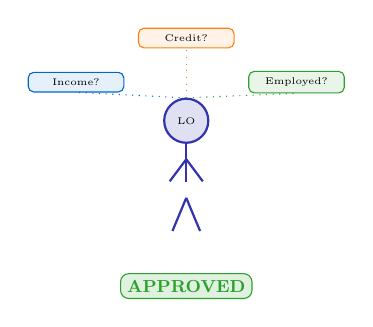
\begin{tikzpicture}[scale=0.7, every node/.style={transform shape}]
% Loan officer
\node[circle, draw=mlpurple, fill=mlpurple!15, minimum size=8mm, line width=0.8pt] (lo) at (0,3.5) {};
\node[font=\tiny] at (0,3.5) {LO};
\draw[mlpurple, line width=0.8pt] (lo.south) -- ++(0,-0.7);
\draw[mlpurple, line width=0.8pt] (-0.3,2.4) -- (0,2.8) -- (0.3,2.4);
\draw[mlpurple, line width=0.8pt] (0,2.1) -- (-0.25,1.5);
\draw[mlpurple, line width=0.8pt] (0,2.1) -- (0.25,1.5);
% Thought bubbles
\node[rounded corners=2pt, draw=mlblue, fill=mlblue!10, font=\tiny, text width=1.5cm, align=center] (b1) at (-2,4.2) {Income?};
\node[rounded corners=2pt, draw=mlorange, fill=mlorange!10, font=\tiny, text width=1.5cm, align=center] (b2) at (0,5) {Credit?};
\node[rounded corners=2pt, draw=mlgreen, fill=mlgreen!10, font=\tiny, text width=1.5cm, align=center] (b3) at (2,4.2) {Employed?};
\draw[mlblue, line width=0.4pt, dotted] (lo.north) -- (b1.south);
\draw[mlorange, line width=0.4pt, dotted] (lo.north) -- (b2.south);
\draw[mlgreen, line width=0.4pt, dotted] (lo.north) -- (b3.south);
% Decision
\node[rounded corners=3pt, draw=mlgreen, fill=mlgreen!15, font=\small\bfseries, text=mlgreen] at (0,0.5) {APPROVED};
\end{tikzpicture}
\end{columns}
\bottomnote{Decision trees formalize this human process: learn the best questions from data}
\end{frame}

%% SLIDE 3: Learning Objectives
\begin{frame}[t]{What Will You Learn in This Lecture?}
\small
\textbf{Learning Objectives}
\begin{enumerate}
\item \footnotesize \highlight{Derive} Gini impurity and information gain from first principles
\item \footnotesize \highlight{Analyze} how recursive partitioning builds axis-aligned boundaries
\item \footnotesize \highlight{Evaluate} overfitting using pruning strategies and cross-validation
\item \footnotesize \highlight{Compare} decision trees with linear models for structured data
\end{enumerate}

\vspace{4mm}
\begin{columns}[T]
\column{0.48\textwidth}
\begin{block}{Prerequisites}
\footnotesize Basic probability, linear/logistic regression concepts (L01--L02).
\end{block}

\column{0.48\textwidth}
\begin{block}{Why It Matters}
\footnotesize DTs are the foundation for Random Forests, XGBoost, and LightGBM.
\end{block}
\end{columns}
\bottomnote{Bloom's levels: derive (4), analyze (4), evaluate (5), compare (5)}
\end{frame}

%% SLIDE 4: Plain English Definition
\begin{frame}[t]{What Is a Decision Tree in Plain English?}
\begin{columns}[T]
\column{0.50\textwidth}
\small
\textbf{A flowchart that learns from data}

\footnotesize
Think of the ``20 Questions'' game: each question narrows down the possibilities. A decision tree does the same --- but \highlight{learns which questions to ask} by analyzing labeled data.
\begin{compactlist}
\item \footnotesize No assumed functional form (non-parametric)
\item \footnotesize Works with numerical and categorical features
\item \footnotesize Each prediction has a human-readable path
\end{compactlist}

\column{0.48\textwidth}
\vspace{2mm}
\footnotesize
\textbf{Vocabulary}
\begin{compactlist}
\item \footnotesize \textbf{Root:} first question (most informative)
\item \footnotesize \textbf{Internal node:} each decision point
\item \footnotesize \textbf{Leaf:} final prediction
\item \footnotesize \textbf{Split:} test that divides data
\item \footnotesize \textbf{Depth:} levels from root to deepest leaf
\item \footnotesize \textbf{Branch:} one path from root to leaf
\end{compactlist}
\end{columns}
\bottomnote{Unlike linear models, decision trees can capture interactions and non-linearities automatically}
\end{frame}

%% SLIDE 5: Where DTs Fit in ML
\begin{frame}[t]{Where Do Decision Trees Fit in Machine Learning?}
\begin{columns}[T]
\column{0.50\textwidth}
\small
\textbf{Parametric vs Non-Parametric}

\vspace{1mm}
\footnotesize
\begin{adjustbox}{max width=\columnwidth}
\begin{tabular}{lcc}
\toprule
& \textbf{Parametric} & \textbf{Non-Parametric} \\
\midrule
Example & Linear/Logistic Reg. & Decision Trees \\
\rowcolor{mllavender4}
Assumption & Fixed form & Data-driven \\
\# Parameters & Fixed & Grows with data \\
\rowcolor{mllavender4}
Interpretability & Coefficients & Decision paths \\
\bottomrule
\end{tabular}
\end{adjustbox}

\vspace{3mm}
\begin{block}{Bridge}
\footnotesize Decision trees are the \highlight{building blocks for Random Forests} (next lecture).
\end{block}

\column{0.48\textwidth}
\footnotesize
\textbf{The ML Landscape So Far}
\begin{compactlist}
\item \footnotesize L01: Linear Regression $\to$ continuous prediction
\item \footnotesize L02: Logistic Regression $\to$ probability + classification
\item \footnotesize L03: KNN/K-Means $\to$ instance-based + clustering
\item \footnotesize \textbf{L04: Decision Trees} $\to$ rule-based, non-linear
\end{compactlist}
\end{columns}
\bottomnote{DTs bridge interpretability (like linear models) and flexibility (like KNN)}
\end{frame}

%% ================================================================
%% CORE ZONE -- METHOD (Slides 6--14)
%% ================================================================

%% SLIDE 6: Non-linear Motivation
\begin{frame}[t]{Why Can't a Straight Line Separate These Borrowers?}
\begin{columns}[T]
\column{0.45\textwidth}
\small
\textbf{The Non-Linearity Problem}

\footnotesize
Some classification problems cannot be solved with a single linear boundary. The XOR-like pattern on the right shows two classes interleaved:
\begin{compactlist}
\item \footnotesize A diagonal line misclassifies many points
\item \footnotesize But two axis-aligned splits at $x=2.5$ and $y=2.5$ separate perfectly
\item \footnotesize Decision trees excel at this
\end{compactlist}

\column{0.53\textwidth}
\vspace{2mm}

\includegraphics[width=0.65\textwidth]{12_nonlinear_classes/chart.pdf}
\end{columns}
\bottomnote{DTs create axis-aligned rectangles --- any non-linear boundary can be approximated with enough splits}
\end{frame}

%% SLIDE 7: What a Trained Tree Looks Like
\begin{frame}[t]{What Does a Trained Decision Tree Look Like?}
\begin{columns}[T]
\column{0.45\textwidth}
\small
\textbf{Anatomy of a Trained Tree}

\footnotesize
\begin{compactlist}
\item \footnotesize \textbf{Root} (top): the most informative split
\item \footnotesize \textbf{Branches}: conditions that route data left or right
\item \footnotesize \textbf{Leaves} (bottom): final class predictions
\item \footnotesize Each path = one interpretable rule
\end{compactlist}
\vspace{2mm}
\begin{block}{Insight}
\footnotesize The tree on the right was trained on fraud detection data --- follow any path from root to leaf to read the decision rule.
\end{block}

\column{0.53\textwidth}
\vspace{2mm}

\includegraphics[width=0.65\textwidth]{01_decision_tree/chart.pdf}
\end{columns}
\bottomnote{sklearn's \texttt{export\_text()} prints the full tree as readable if/else rules}
\end{frame}

%% SLIDE 8: Gini Impurity Formula
\begin{frame}[t]{How Does the Tree Choose the Best Split? (Gini Impurity)}
\small
\textbf{Gini Impurity Formula}

\vspace{1mm}
\footnotesize
For a node with $K$ classes and class proportions $p_1, p_2, \ldots, p_K$:
\[
G(p) = 1 - \sum_{k=1}^{K} p_k^2
\]

\textbf{Worked example:} 100 loan applicants, 60 repay, 40 default.
\[
G = 1 - (0.6^2 + 0.4^2) = 1 - (0.36 + 0.16) = 1 - 0.52 = \highlight{0.48}
\]

\begin{columns}[T]
\column{0.48\textwidth}
\begin{block}{Interpretation}
\footnotesize $G = 0$ means pure node (all one class). $G = 0.5$ means maximum impurity for 2 classes.
\end{block}

\column{0.48\textwidth}
\begin{block}{Intuition}
\footnotesize Gini = probability that a randomly chosen sample would be \textbf{misclassified} if labeled by the node's distribution.
\end{block}
\end{columns}
\bottomnote{Binary Gini: $G = 2p(1-p)$, peaks at $p = 0.5$}
\end{frame}

%% SLIDE 9: Which Split Reduces Impurity Most
\begin{frame}[t]{Which Split Reduces Impurity the Most?}
\begin{columns}[T]
\column{0.50\textwidth}
\small
\textbf{Weighted Gini After Split}

\footnotesize
Parent: 100 applicants (60/40), $G = 0.48$.

After splitting on ``Income > \$50k'':
\begin{compactlist}
\item \footnotesize Left child: 40 apps (70/30) $\to G = 0.42$
\item \footnotesize Right child: 60 apps (90/10) $\to G = 0.18$
\end{compactlist}

\vspace{1mm}
Weighted average:
\[
G_{\text{weighted}} = \frac{40}{100} \times 0.42 + \frac{60}{100} \times 0.18 = \highlight{0.276}
\]

Impurity reduction:
\[
\Delta G = 0.48 - 0.276 = \highlight{0.204}
\]

\column{0.48\textwidth}
\vspace{2mm}

\includegraphics[width=0.55\textwidth]{08_gini_split/chart.pdf}
\end{columns}
\bottomnote{The tree greedily picks the feature and threshold that maximize $\Delta G$ at each node}
\end{frame}

%% SLIDE 10: Entropy
\begin{frame}[t]{What Does Entropy Add Beyond Gini?}
\begin{columns}[T]
\column{0.50\textwidth}
\small
\textbf{Entropy (Information Theory)}

\footnotesize
\[
H(p) = -\sum_{k=1}^{K} p_k \log_2 p_k
\]

\textbf{Same example:} 60 repay, 40 default.
\[
H = -(0.6 \log_2 0.6 + 0.4 \log_2 0.4) = \highlight{0.971 \text{ bits}}
\]

\begin{compactlist}
\item \footnotesize $H = 0$ for pure node, $H = 1$ for 50/50 binary
\item \footnotesize Entropy penalizes impurity slightly more than Gini
\item \footnotesize In practice, both produce nearly identical trees
\end{compactlist}

\column{0.48\textwidth}
\vspace{2mm}

\includegraphics[width=0.55\textwidth]{11_gini_vs_entropy/chart.pdf}
\end{columns}
\bottomnote{sklearn default is Gini; use \texttt{criterion='entropy'} to switch}
\end{frame}

%% SLIDE 11: Information Gain
\begin{frame}[t]{Information Gain: The Decision Rule}
\small
\textbf{Information Gain = Entropy Before $-$ Weighted Entropy After}

\vspace{1mm}
\footnotesize
\[
\text{IG}(D, \text{feature}) = H(D) - \sum_{v \in \text{values}} \frac{|D_v|}{|D|} \times H(D_v)
\]

\textbf{Worked example with 2 candidate features:}
\begin{columns}[T]
\column{0.48\textwidth}
\textbf{Split on Income ($> \$50$k):}
\begin{compactlist}
\item \footnotesize Left: 40 apps, $H = 0.881$
\item \footnotesize Right: 60 apps, $H = 0.469$
\item \footnotesize $\text{IG} = 0.971 - (0.4 \times 0.881 + 0.6 \times 0.469)$
\item \footnotesize $\text{IG} = 0.971 - 0.634 = \highlight{0.337}$
\end{compactlist}

\column{0.48\textwidth}
\textbf{Split on Employment ($> 2$yr):}
\begin{compactlist}
\item \footnotesize Left: 50 apps, $H = 0.722$
\item \footnotesize Right: 50 apps, $H = 0.722$
\item \footnotesize $\text{IG} = 0.971 - (0.5 \times 0.722 + 0.5 \times 0.722)$
\item \footnotesize $\text{IG} = 0.971 - 0.722 = \highlight{0.249}$
\end{compactlist}
\end{columns}

\vspace{2mm}
\begin{block}{Decision}
\footnotesize Income wins ($\text{IG} = 0.337 > 0.249$) $\to$ split on Income first.
\end{block}
\bottomnote{ID3 uses information gain; C4.5 uses gain ratio to correct for multi-valued features}
\end{frame}

%% SLIDE 12: Decision Boundaries
\begin{frame}[t]{How Does the Tree Partition Feature Space?}
\begin{columns}[T]
\column{0.45\textwidth}
\small
\textbf{Axis-Aligned Rectangles}

\footnotesize
Each split creates a horizontal or vertical boundary in feature space. After depth 3:
\begin{compactlist}
\item \footnotesize Up to $2^3 = 8$ rectangular regions
\item \footnotesize Each rectangle = one leaf node
\item \footnotesize More depth = finer rectangles = risk of overfit
\end{compactlist}
\vspace{2mm}
\begin{block}{Limitation}
\footnotesize DTs can only make axis-aligned cuts --- diagonal boundaries need many splits to approximate.
\end{block}

\column{0.53\textwidth}
\vspace{2mm}

\includegraphics[width=0.65\textwidth]{10_dt_decision_boundary/chart.pdf}
\end{columns}
\bottomnote{Each rectangle corresponds to a path: ``if $x_1 > a$ AND $x_2 \leq b$ then class = \ldots''}
\end{frame}

%% SLIDE 13: Recursive Partitioning Algorithm
\begin{frame}[fragile,t]{The Recursive Partitioning Algorithm}
\small
\textbf{GROW-TREE: How the Algorithm Works}

\vspace{1mm}
\footnotesize
\begin{algorithmic}[1]
\REQUIRE Dataset $D$, feature set $F$, max depth $d$
\ENSURE A decision tree $T$
\IF{all samples in $D$ have same label OR $d = 0$ OR $|D| < $ min\_samples}
  \RETURN leaf with majority class
\ENDIF
\STATE $f^*, t^* \gets$ feature and threshold maximizing $\Delta G$ (or IG)
\STATE $D_L \gets \{x \in D : x_{f^*} \leq t^*\}$
\STATE $D_R \gets \{x \in D : x_{f^*} > t^*\}$
\STATE left $\gets$ \textsc{Grow-Tree}($D_L$, $F$, $d-1$)
\STATE right $\gets$ \textsc{Grow-Tree}($D_R$, $F$, $d-1$)
\RETURN node with split $(f^*, t^*)$, left, right
\end{algorithmic}

\vspace{2mm}
\begin{block}{Key Point}
\footnotesize Greedy: each split is locally optimal. No backtracking --- finding the globally optimal tree is NP-hard.
\end{block}
\bottomnote{Time complexity: $O(n \cdot p \cdot d)$ where $n$ = samples, $p$ = features, $d$ = depth}
\end{frame}

%% SLIDE 14: Stopping Rules
\begin{frame}[t]{What Are the Stopping Rules?}
\small
\textbf{When Does the Tree Stop Growing?}

\vspace{2mm}
\footnotesize
\begin{adjustbox}{max width=\textwidth}
\begin{tabular}{lp{5cm}p{5cm}}
\toprule
\textbf{Parameter} & \textbf{Effect} & \textbf{Trade-off} \\
\midrule
\texttt{max\_depth} & Limits tree levels & \footnotesize Too low $\to$ underfit; too high $\to$ overfit \\
\rowcolor{mllavender4}
\texttt{min\_samples\_leaf} & Minimum samples in a leaf & \footnotesize Higher = smoother; lower = noisier \\
\texttt{min\_impurity\_decrease} & Minimum $\Delta G$ to split & \footnotesize Prunes weak splits early \\
\rowcolor{mllavender4}
\texttt{max\_leaf\_nodes} & Caps number of leaves & \footnotesize Controls model complexity \\
\bottomrule
\end{tabular}
\end{adjustbox}

\vspace{3mm}
\begin{block}{Insight}
\footnotesize These are \highlight{pre-pruning} strategies --- they prevent overfitting before it happens.
\end{block}
\bottomnote{Use cross-validation to select optimal values for each stopping parameter}
\end{frame}

%% ================================================================
%% CORE ZONE -- SOLUTION (Slides 15--19)
%% ================================================================

%% SLIDE 15: Interpreting Paths
\begin{frame}[t]{Interpreting the Tree: What Does Each Path Mean?}
\small
\textbf{Three Loan Applicants Through the Tree}

\vspace{1mm}
\footnotesize
\begin{adjustbox}{max width=\textwidth}
\begin{tabular}{clp{7cm}c}
\toprule
\textbf{Applicant} & \textbf{Path} & \textbf{Interpretable Rule} & \textbf{Decision} \\
\midrule
A & Income $> 50$k $\to$ Credit $> 680$ & \footnotesize High income AND good credit & \textcolor{mlgreen}{\textbf{Approve}} \\
\rowcolor{mllavender4}
B & Income $\leq 50$k $\to$ Employment $> 2$yr & \footnotesize Low income BUT stable job & \textcolor{mlgreen}{\textbf{Approve}} \\
C & Income $\leq 50$k $\to$ Employment $\leq 2$yr & \footnotesize Low income AND short tenure & \textcolor{dfred}{\textbf{Deny}} \\
\bottomrule
\end{tabular}
\end{adjustbox}

\vspace{3mm}
\begin{columns}[T]
\column{0.48\textwidth}
\begin{block}{Key Advantage}
\footnotesize Every prediction comes with a \highlight{reason} --- critical for regulated industries.
\end{block}

\column{0.48\textwidth}
\begin{block}{Limitation}
\footnotesize Interpretability fades as depth increases --- a 20-level path is hard to explain.
\end{block}
\end{columns}
\bottomnote{ECOA requires lenders to explain adverse actions --- DT paths provide natural explanations}
\end{frame}

%% SLIDE 16: Feature Importance
\begin{frame}[t]{Reading Feature Importance from a Single Tree}
\begin{columns}[T]
\column{0.55\textwidth}
\small
\textbf{Mean Decrease in Impurity (MDI)}

\footnotesize
\begin{compactlist}
\item \footnotesize Features used near the \highlight{root} contribute the most impurity reduction
\item \footnotesize MDI sums $\Delta G$ across all nodes where a feature is used, weighted by samples
\item \footnotesize Normalized so all importances sum to 1
\end{compactlist}

\vspace{2mm}
\textbf{Permutation Importance (alternative):}
\begin{compactlist}
\item \footnotesize Shuffle one feature, measure accuracy drop
\item \footnotesize More reliable for correlated features
\item \footnotesize Slower but unbiased
\end{compactlist}

\column{0.42\textwidth}
\vspace{2mm}
\begin{block}{Comparison}
\footnotesize
\begin{tabular}{lcc}
\toprule
& \textbf{MDI} & \textbf{Permutation} \\
\midrule
Speed & Fast & Slow \\
Bias & High-card. & Unbiased \\
Scope & Train & Test \\
\bottomrule
\end{tabular}
\end{block}
\end{columns}
\bottomnote{MDI overestimates importance of high-cardinality features --- always cross-check with permutation}
\end{frame}

%% SLIDE 17: Overfitting and Pruning
\begin{frame}[t]{The Overfitting Problem: Why Deep Trees Memorize}
\small
\textbf{Pre-Pruning vs Post-Pruning}

\vspace{1mm}
\footnotesize
\begin{columns}[T]
\column{0.48\textwidth}
\textbf{Pre-Pruning (stop early):}
\begin{compactlist}
\item \footnotesize Set \texttt{max\_depth}, \texttt{min\_samples\_leaf}
\item \footnotesize Fast but may stop too soon
\item \footnotesize Used by sklearn's \texttt{DecisionTreeClassifier}
\end{compactlist}

\column{0.48\textwidth}
\textbf{Post-Pruning (grow then cut):}
\begin{compactlist}
\item \footnotesize Grow full tree, then remove branches
\item \footnotesize Cost-complexity pruning (CCP):
\end{compactlist}
\end{columns}

\vspace{2mm}
\[
R_\alpha(T) = R(T) + \alpha \cdot |T|
\]
\footnotesize
where $R(T)$ = misclassification rate, $|T|$ = number of leaves, $\alpha$ = complexity penalty.

\vspace{2mm}
\begin{block}{Insight}
\footnotesize Increasing $\alpha$ prunes more aggressively --- use CV to find optimal $\alpha$.
\end{block}
\bottomnote{sklearn: use \texttt{ccp\_alpha} parameter and \texttt{cost\_complexity\_pruning\_path()} to find candidates}
\end{frame}

%% SLIDE 18: Train/Test Error Chart
\begin{frame}[t]{Can You See the Overfitting?}
\begin{columns}[T]
\column{0.50\textwidth}
\small
\textbf{Depth vs Error}

\footnotesize
\begin{compactlist}
\item \footnotesize Train error drops monotonically as depth increases
\item \footnotesize Test error drops, then \highlight{rises} --- classic overfitting
\item \footnotesize Optimal depth: where test error is minimized
\item \footnotesize Use $k$-fold cross-validation to select depth
\end{compactlist}

\vspace{2mm}
\begin{block}{Insight}
\footnotesize The gap between train and test error is a direct measure of overfitting.
\end{block}

\column{0.48\textwidth}
\vspace{2mm}

\includegraphics[width=0.55\textwidth]{09_dt_overfitting/chart.pdf}
\end{columns}
\bottomnote{sklearn: \texttt{GridSearchCV(param\_grid=\{`max\_depth': range(1,20)\})} automates this}
\end{frame}

%% SLIDE 19: Regression Trees
\begin{frame}[t]{Regression Trees: Predicting Numbers, Not Categories}
\small
\textbf{MSE Instead of Gini}

\vspace{1mm}
\footnotesize
For regression, each leaf predicts the \highlight{mean} of its samples. The split criterion becomes:
\[
\text{MSE}(D) = \frac{1}{|D|} \sum_{i \in D} (y_i - \bar{y})^2
\]

\textbf{Worked example:} Predict house price.
\begin{columns}[T]
\column{0.48\textwidth}
\begin{compactlist}
\item \footnotesize Parent: 10 houses, mean price = \$300k, MSE = 5000
\item \footnotesize Split on sqft $> 1500$:
\item \footnotesize Left: 4 houses, mean = \$200k, MSE = 1200
\item \footnotesize Right: 6 houses, mean = \$367k, MSE = 800
\end{compactlist}

\column{0.48\textwidth}
\begin{compactlist}
\item \footnotesize Weighted MSE = $\frac{4}{10} \times 1200 + \frac{6}{10} \times 800 = 960$
\item \footnotesize Reduction = $5000 - 960 = 4040$
\end{compactlist}
\vspace{2mm}
\begin{block}{Key}
\footnotesize Same algorithm, different criterion: minimize variance instead of impurity.
\end{block}
\end{columns}
\bottomnote{sklearn: \texttt{DecisionTreeRegressor(criterion='squared\_error')}}
\end{frame}

% Regression Tree MSE Split (chart)
\begin{frame}[t]{Regression Trees: MSE Split Visualization}
\begin{center}

\includegraphics[width=0.65\textwidth]{16_regression_tree_mse/chart.pdf}
\end{center}
\bottomnote{A depth-1 regression tree finds the optimal split that minimizes weighted MSE in child nodes}
\end{frame}

%% ================================================================
%% CLOSING ZONE (Slides 20--25)
%% ================================================================

%% SLIDE 20: When to Use DT
\begin{frame}[t]{When to Use a Decision Tree --- and When Not To}
\small
\begin{columns}[T]
\column{0.48\textwidth}
\textbf{\textcolor{mlgreen}{Pros}}
\begin{compactlist}
\item \footnotesize Interpretable decision paths
\item \footnotesize Handles mixed feature types
\item \footnotesize No feature scaling needed
\item \footnotesize Fast training and prediction
\end{compactlist}

\column{0.48\textwidth}
\textbf{\textcolor{dfred}{Cons}}
\begin{compactlist}
\item \footnotesize High variance (unstable)
\item \footnotesize Prone to overfitting
\item \footnotesize Axis-aligned boundaries only
\item \footnotesize Small changes in data $\to$ different tree
\end{compactlist}
\end{columns}

\vspace{3mm}
\begin{block}{Bridge to Random Forests}
\footnotesize The solution to high variance: \highlight{grow many trees and let them vote} $\to$ Random Forests (next lecture).
\end{block}
\bottomnote{A single tree is rarely used in production --- it is a building block for ensembles}
\end{frame}

%% SLIDE 21: DT vs Logistic Regression
\begin{frame}[t]{DT vs Logistic Regression for Credit Scoring}
\small
\textbf{Head-to-Head Comparison}

\vspace{2mm}
\footnotesize
\begin{adjustbox}{max width=\textwidth}
\begin{tabular}{lcc}
\toprule
\textbf{Property} & \textbf{Decision Tree} & \textbf{Logistic Regression} \\
\midrule
Decision boundary & Axis-aligned rectangles & Linear hyperplane \\
\rowcolor{mllavender4}
Feature interactions & Captured automatically & Must engineer manually \\
Interpretability & Path-based rules & Odds ratios \\
\rowcolor{mllavender4}
Probability output & Leaf proportions (noisy) & Calibrated via sigmoid \\
Stability & Low (high variance) & High (low variance) \\
\rowcolor{mllavender4}
Missing values & Can handle natively & Requires imputation \\
Non-linearity & Built-in & Requires feature transforms \\
\bottomrule
\end{tabular}
\end{adjustbox}

\vspace{2mm}
\begin{block}{When to Choose Which}
\footnotesize Regulated setting with linear relationships $\to$ logistic regression. Complex interactions $\to$ DT or RF.
\end{block}
\bottomnote{Many teams use both: logistic regression for baseline, DT/RF for production}
\end{frame}

%% SLIDE 22: Hands-on Exercise
\begin{frame}[fragile,t]{Hands-on: Build a Credit Scoring Tree}
\small
\textbf{Exercise with sklearn}

\vspace{1mm}
\footnotesize
\begin{columns}[T]
\column{0.48\textwidth}
\textbf{Step 1: Load and split}
\begin{verbatim}
from sklearn.tree import (
    DecisionTreeClassifier,
    export_text)
from sklearn.model_selection import (
    train_test_split)

X_train, X_test, y_train, y_test = \
    train_test_split(X, y,
    test_size=0.3, random_state=42)
\end{verbatim}

\column{0.48\textwidth}
\textbf{Step 2: Train and evaluate}
\begin{verbatim}
clf = DecisionTreeClassifier(
    max_depth=4,
    min_samples_leaf=10,
    random_state=42)
clf.fit(X_train, y_train)

print(f"Test acc: "
  f"{clf.score(X_test, y_test):.3f}")
print(export_text(clf,
  feature_names=feat_names))
\end{verbatim}
\end{columns}

\vspace{2mm}
\begin{block}{Tasks}
\footnotesize (1) Vary \texttt{max\_depth} from 1 to 15 and plot train/test accuracy. (2) Find optimal depth via CV.
\end{block}
\bottomnote{Use \texttt{plot\_tree(clf)} to visualize --- or \texttt{export\_graphviz} for publication-quality figures}
\end{frame}

%% SLIDE 23: Key Takeaways
\begin{frame}[t]{Key Takeaways}
\small
\begin{columns}[T]
\column{0.48\textwidth}
\textbf{Concepts}
\begin{compactlist}
\item \footnotesize \highlight{Gini impurity}: $G = 1 - \sum p_k^2$
\item \footnotesize \highlight{Entropy}: $H = -\sum p_k \log_2 p_k$
\item \footnotesize \highlight{Information gain}: parent entropy minus weighted child entropy
\item \footnotesize \highlight{Recursive partitioning}: greedy, top-down
\item \footnotesize \highlight{Pruning}: pre- and post- to control depth
\end{compactlist}

\column{0.48\textwidth}
\textbf{Practical Skills}
\begin{compactlist}
\item \footnotesize Interpret paths as decision rules
\item \footnotesize Choose depth via cross-validation
\item \footnotesize Read feature importance (MDI + permutation)
\item \footnotesize When to use DT vs logistic regression
\item \footnotesize DTs $\to$ building blocks for RF
\end{compactlist}
\end{columns}
\vspace{3mm}
\begin{block}{One-Sentence Summary}
\footnotesize A decision tree learns the best sequence of yes/no questions from data, trading interpretability for variance.
\end{block}
\bottomnote{Master decision trees and you have the foundation for all tree-based ensemble methods}
\end{frame}

%% SLIDE 24: Bridge to Random Forests
\begin{frame}[t]{What's Next: From One Tree to a Forest}
\small
\textbf{The Problem with One Tree}

\footnotesize
\begin{compactlist}
\item \footnotesize A single tree is \highlight{unstable}: small data changes $\to$ completely different tree
\item \footnotesize High variance limits practical accuracy
\item \footnotesize The fix: \textbf{grow 500 different trees and let them vote}
\end{compactlist}

\vspace{3mm}
\begin{columns}[T]
\column{0.48\textwidth}
\begin{block}{Random Forest Recipe}
\footnotesize
\begin{enumerate}
\item Bootstrap sample the data
\item At each split, use $\sqrt{p}$ random features
\item Grow many decorrelated trees
\item Aggregate by majority vote
\end{enumerate}
\end{block}

\column{0.48\textwidth}
\begin{block}{Why It Works}
\footnotesize
\[
\text{Var}(\bar{f}) = \rho\sigma^2 + \frac{1-\rho}{B}\sigma^2
\]
Decorrelating trees ($\rho \downarrow$) reduces ensemble variance.
\end{block}
\end{columns}
\bottomnote{Next lecture: Random Forests --- bagging, feature randomization, OOB error, feature importance}
\end{frame}

%% SLIDE 25: Closing Thought + XKCD
\begin{frame}[t]{Closing Thought}
\begin{columns}[T]
\column{0.50\textwidth}
\vspace{4mm}
\small
\textbf{``The tree that learns too well from the past is doomed to fail in the future.''}

\vspace{4mm}
\footnotesize
Decision trees teach us the fundamental trade-off in machine learning: \highlight{complexity vs generalization}. Every additional split fits the training data better --- but risks memorizing noise.

\vspace{3mm}
The solution? Don't trust one tree. Trust a forest.

\column{0.48\textwidth}
\vspace{2mm}
\centering

\includegraphics[height=0.45\textheight]{images/1838_machine_learning.png}
\end{columns}
\bottomnote{XKCD \#1838 by Randall Munroe (CC BY-NC 2.5)}
\end{frame}

\end{document}
